% 1977 年黑龙江初试卷第 11 题：△ABC 中 ∠A=120°，∠B=45°，AC=6cm（按源卷第 3 页布局）
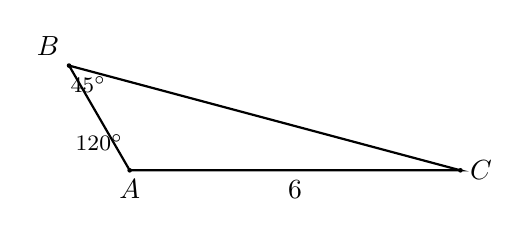
\begin{tikzpicture}[scale=0.7]
  \coordinate (A) at (0,0);
  \coordinate (C) at (6,0);
  \coordinate (B) at (-1.1,1.9);
  \draw[thick] (A)--(B)--(C)--cycle;
  \fill (A) circle (1.2pt) node[below] {$A$};
  \fill (B) circle (1.2pt) node[above left] {$B$};
  \fill (C) circle (1.2pt) node[right] {$C$};
  \node at (-0.55,0.5) {\footnotesize $120^\circ$};
  \node at (-0.75,1.55) {\footnotesize $45^\circ$};
  \node at (3,-0.35) {$6$};
\end{tikzpicture}
